\documentclass[a4,11pt]{aleph-notas}
% Se puede ver la documentación aquí: 
% https://github.com/alephsub0/LaTeX_aleph-notas

% -- Paquetes adicionales
\usepackage{enumitem}
\usepackage{aleph-comandos}
\usepackage{booktabs}

\usepackage{amsmath}
\usepackage{pgfplots}
\pgfplotsset{compat=1.18}



% -- Datos 
\institucion{Escuela de Ciencias Físicas y Matemática}
\carrera{Medicina Veterinaria}
\asignatura{Matemática I*}
\tema{Resumen no. 3: Funciones: definición, propiedades y aplicaciones}
\autor{Alejandro Galvis}
\fecha{Semestre 2024-2}

\logouno[0.14\textwidth]{Logos/logoPUCE_04_ac}
\definecolor{colortext}{HTML}{0030A1}
\definecolor{colordef}{HTML}{0030A1}
\fuente{montserrat}


% -- Comandos adicionales
\setlist[enumerate]{label=\roman*.}
\definecolor{colcod}{RGB}{174,218,255}
\newtcolorbox{pycodigo}
    {icono=\faKeyboardO,color=colcod,postit,top=2mm,bottom=2mm}


\begin{document}

\encabezado

%%%%%%%%%%%%%%%%%%%%%%%%%%%%%%%%%%%%%%%
\section{Definición de función}
%%%%%%%%%%%%%%%%%%%%%%%%%%%%%%%%%%%%%%%

El concepto de \textbf{función} es el más importante en matemática.
\begin{itemize}
    \item Dan lugar a la construcción de una gran cantidad de estructuras que constituyen la base para el desarrollo de muchas áreas de la matemática.
    \item Juegan un papel primordial en la modelación de situaciones de la vida real.
    \item Todos los que utilizan la Matemática, esencialmente estudian funciones: físicos, biólogos, economistas, psicólogos, ingenieros, entre otros.
    \item Una función es una relación, lo contrario no siempre es cierto.
    \item Se debe precisar que una magnitud es cualquier característica que puede ser medida y su valor expresado mediante un número.    
\end{itemize}

\vspace{1pt}
\begin{defi}[Función]
    Se denomina \textbf{función real} de $A$ en $B$ a la correspondencia entre dos conjuntos de números reales, $\mathbb{R}$, de forma que a cada elemento $x$ del conjunto $A$, le corresponde un único elemento $y$ del conjunto $B$.
\end{defi}

\begin{advertencia}
    Si $f$ es una función de $A$ en $B$, escribirá $\func{f}{A}{B}$. Y, si a un elemento $x$ de $A$ le corresponde el elemento $y$ de $B$, se escribe $f(x)=y$.
\end{advertencia}

\begin{obs}
    No toda correspondencia es función.
\end{obs}

Veamos dos ejemplos de funciones en Medicina Veterinaria:

\begin{ejem}[Relación entre peso y dosis de medicamento]
    Una función común en medicina veterinaria es la relación entre el peso de un animal y la dosis de medicamento que se le debe administrar. Supongamos que se tiene una fórmula donde la dosis  $D$ (en mililitros) de un medicamento depende del peso $P$ (en kilogramos) de un animal. La función podría representarse como:
    \[ 
        D(P) = 0.05 \cdot P.
    \]
    En este caso, para un animal que pesa 10 kg, la dosis será:
    \[
        D(10) = 0.05 \times 10 = 0.5 \, \text{ml}.
    \]
\end{ejem}

\begin{ejem}[Crecimiento de un cachorro]

    En estudios de crecimiento de animales, como los cachorros, el peso de un cachorro $P(t)$ puede ser una función del tiempo $t$ (en semanas). Por ejemplo, si un cachorro gana 2 kg por semana, la función que modela su crecimiento podría ser:
    \[
        P(t) = 5 + 2t,
    \]
    donde \( 5 \, \text{kg} \) es el peso inicial del cachorro al nacer y \( t \) es el número de semanas desde el nacimiento. A las 4 semanas, el peso del cachorro sería:
    \[
        P(4) = 5 + 2 \times 4 = 13 \, \text{kg}.
    \]
\end{ejem}

%%%%%%%%%%%%%%%%%%%%%%%%%%%%%%%%%%%%%%%
\section{Representación de funciones}
%%%%%%%%%%%%%%%%%%%%%%%%%%%%%%%%%%%%%%%

Una función se puede representar mediante un texto, mediante una fórmula algebraica, por una tabla de valores o a través de un gráfico. Además existe un conjunto básico de funciones que por su uso frecuente en muchas aplicaciones es necesario reconocer y analizar.

\subsection*{Función Lineal}

\begin{defi}[Función lineal]
    Dados $a \in \R$ y $b\in\R$, una \textbf{función lineal} es la que tiene la forma:
    \[
        \funcion{f}{\R}{\R}{x}{ax+b.}
    \]
\end{defi}

\subsubsection*{Ejemplo de representación textual}

Una función lineal relaciona el costo de una consulta veterinaria con el número de consultas realizadas. Si cada consulta cuesta \$50, el costo total es proporcional al número de consultas.

\subsubsection*{Ejemplo de representación Algebraica}
La función es
\[
    \funcion{f}{\R}{\R}{x}{f(x) = 50x,}
\]
donde $x$ es el número de consultas y $f(x)$ es el costo total en dólares.

\subsubsection*{Ejemplo de representación Tabular}

\begin{center}\small
\begin{tabular}{@{}cc@{}}
\toprule
Número de Consultas & Costo Total \\
$x$ & $f(x)$\\
\midrule
1 & 50 \\
2 & 100 \\
3 & 150 \\
4 & 200 \\
5 & 250 \\
\bottomrule
\end{tabular}
\end{center}

\subsubsection*{Ejemplo de representación Gráfica}
\begin{center}
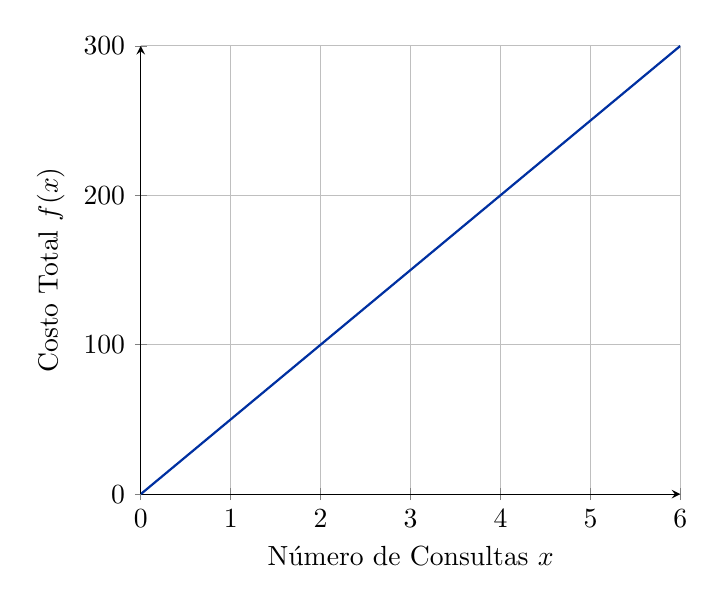
\begin{tikzpicture}
    \begin{axis}[
        axis lines = left,
        xlabel = {Número de Consultas $x$},
        ylabel = {Costo Total $f(x)$},
        ymin=0, ymax=300, xmin=0, xmax=6,
        grid=both,
        domain=0:5,
        samples=100
    ]
    \addplot[color=colordef, thick, domain=0:6]{50*x};
    \end{axis}
\end{tikzpicture}
\end{center}

\subsection*{Función Cuadrática}

\begin{defi}[Función cuadrática]  
Dados $a \in \R \setminus \{0\}$, $b,c\in\R$, una \textbf{función cuadrática} es la que tiene la forma:
\[
\funcion{f}{\R}{\R}{x}{ax^2 + bx + c.}
\]
\end{defi}

\subsubsection*{Ejemplo de Representación Textual}  
La distancia máxima que un gato puede alcanzar al saltar verticalmente depende de la velocidad inicial con la que se impulsa. Esta relación puede modelarse con una función cuadrática, donde la altura máxima alcanzada depende de la velocidad de lanzamiento de forma no lineal. A velocidades muy altas o bajas, la altura disminuye.

\subsubsection*{Ejemplo de Representación Algebraica}  
La altura máxima alcanzada por el gato en función de su velocidad inicial está dada por:  
\[
    f(v) = -5v^2 + 20v,
\]
donde \(v\) es la velocidad inicial en metros por segundo (\(m/s\)) y \(f(v)\) es la altura máxima alcanzada en metros (\(m\)).

\subsubsection*{Ejemplo de Representación Tabular}  
\begin{center}\small
\begin{tabular}{@{}cc@{}}
\toprule
Velocidad Inicial  & Altura Máxima \(f(v)\) (\(m\)) \\
\(v\) (\(m/s\)) & \(f(v)\) (\(m\))\\
\midrule
0 & 0 \\
2 & 20 \\
4 & 40 \\
6 & 30 \\
8 & 0 \\
\bottomrule
\end{tabular}
\end{center}
¿Es correcta la representación?

\subsubsection*{Ejemplo de Representación Gráfica}  
\begin{center}
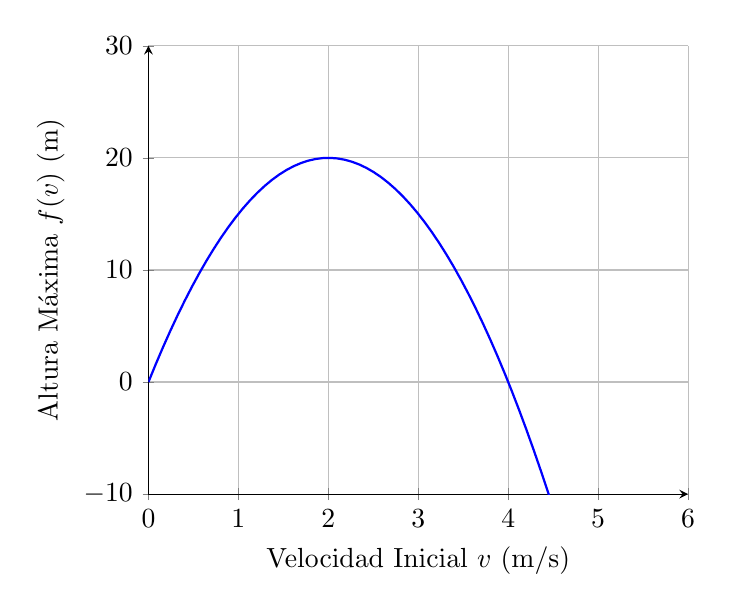
\begin{tikzpicture}
    \begin{axis}[
        axis lines = left,
        xlabel = {Velocidad Inicial \(v\) (m/s)},
        ylabel = {Altura Máxima \(f(v)\) (m)},
        ymin=-10, ymax=30, xmin=0, xmax=6,
        grid=both,
        domain=0:8,
        samples=100
    ]
        \addplot[color=blue, thick]{-5*x^2 + 20*x};
    \end{axis}
\end{tikzpicture}
\end{center}

\subsection*{Función Polinomial y Racional}

\begin{defi}[Función polinómica]
    Dados $n\in \N^*$ y $a_0,\ldots,a_n\in\R$ con $a_n\neq 0$, una \textbf{función polinomial} es la que tiene la forma:
    \[
        \funcion{f}{\R}{\R}{x}{a_nx^n+\cdots+ a_1x+a_0.}
    \]
\end{defi}

\begin{defi}[Función racional]  
    Dadas dos funciones polinomiales \(P(x)\) y \(Q(x)\), una \textbf{función racional} es la que tiene la forma:
    \[
        f(x)=\frac{P(x)}{Q(x)}.
    \]
\end{defi}

\subsubsection*{Ejemplo de Representación Textual}  
La concentración de un medicamento en el cuerpo de un animal varía en función del tiempo y puede describirse con una función racional. Esta función tiene en cuenta tanto la dosis administrada como la tasa de eliminación del medicamento, permitiendo predecir su concentración a lo largo del tiempo.

\subsubsection*{Ejemplo de Representación Algebraica}  
La relación entre el tiempo y la concentración del medicamento se modela mediante:  
\[
f(t) = \frac{3t + 4}{t^2 + 2t + 5},
\]
donde \(t\) representa el tiempo en horas, y \(f(t)\) es la concentración del medicamento en miligramos por mililitro (mg/ml).

\subsubsection*{Ejemplo de Representación Tabular}  
\begin{center}\small
\begin{tabular}{@{}cc@{}}
\toprule
Tiempo  & Concentración  \\
\(t\) (horas) & \(f(t)\) (mg/ml) \\
\midrule
0 & 0.8 \\
1 & 0.875 \\
2 & 0.846 \\
3 & 0.833 \\
4 & 0.818 \\
\bottomrule
\end{tabular}
\end{center}

\subsubsection*{Ejemplo de Representación Gráfica}  
\begin{center}
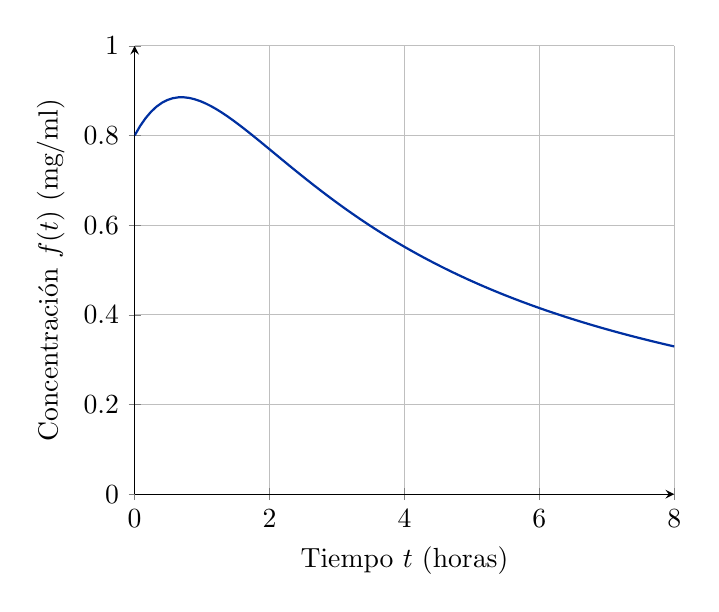
\begin{tikzpicture}
    \begin{axis}[
        axis lines = left,
        xlabel = {Tiempo \(t\) (horas)},
        ylabel = {Concentración \(f(t)\) (mg/ml)},
        ymin=0, ymax=1, xmin=0, xmax=8,
        grid=both,
        domain=0:4,
        samples=100
    ]
        \addplot[color=colordef, thick, domain=0:8]{(3*x + 4) / (x^2 + 2*x + 5)};
    \end{axis}
\end{tikzpicture}
\end{center}

%%%%%%%%%%%%%%%%%%%%%%%%%%%%%%%%%%%%%%%
\section{Un poco de programación en Python}
%%%%%%%%%%%%%%%%%%%%%%%%%%%%%%%%%%%%%%%

%\begin{tcolorbox}[title=¡Importante!]
%    Material recomendado para esta sección acceder al siguiente enlace:\\
%    \href{https://colab.research.google.com/drive/1dtsJCBOb-2m2BGXqca7iavwkilENi69B?usp=sharing}{Notebook de Google Colab}
%\end{tcolorbox}

\begin{pycodigo}
    \textbf{Enlace:} Material recomendado para esta sección acceder a estos enlace
    \begin{itemize}
        \item 
        \href{https://colab.research.google.com/drive/1dtsJCBOb-2m2BGXqca7iavwkilENi69B?usp=sharing}{Notebook de Google Colab}
        \item 
        \href{https://colab.research.google.com/github/ECFM-PUCE/Python-Notebooks-Educativos/blob/main/Representacion-funciones-calculadora.ipynb}{Representación de funciones (calculadora)}
        \item 
        \href{https://colab.research.google.com/github/ECFM-PUCE/Python-Notebooks-Educativos/blob/main/Representacion-funciones-codigo.ipynb}{Representación de funciones (código)}
    \end{itemize}
\end{pycodigo}



\end{document}